\documentclass{article}

\usepackage{hyperref}
\usepackage[T1]{fontenc}
\usepackage{graphicx}
\usepackage[utf8]{inputenc}

\title{Laboratorium 1 - Analiza błędów}
\author{Mateusz Król}
\date{06/03/2024 r.}

\begin{document}
\maketitle


\section*{Zadanie 1.}
\textbf{Oblicz przybliżoną wartość pochodnej funkcji tan(x) dla x = 1.} 
\\\\
Dla wzoru $f'(x)\approx\frac{f(x+h)-f(x)}{h}$, błędy prezentują się następująco:
\begin{figure}[ht!]
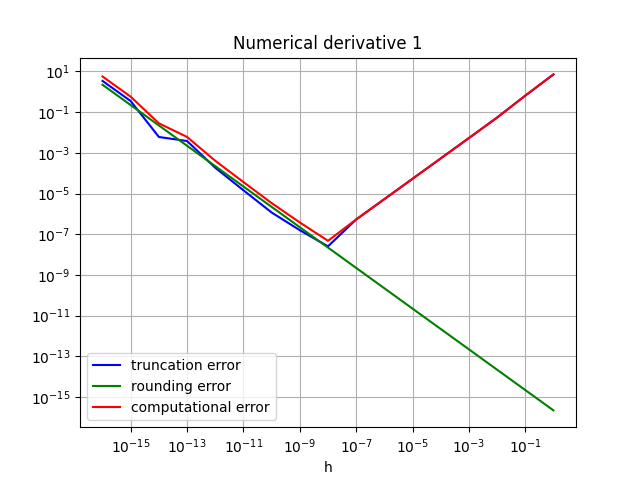
\includegraphics[width=\linewidth]{figures/numerical_derivative_1.png}
\end{figure}
\\

Wyznaczona wartość: $h_{min} = 10^{-8}$ \\
Wartość otrzymana ze wzoru $h_{min} \approx 2\cdot\sqrt[]{\epsilon/M}$,
gdzie $M \approx \left|f''(x)\right|$: \\
$$M\approx \left|\frac{2 \cdot sin(x)}{cos^{3}(x)}\right|
\approx \left|\frac{2 \cdot sin(1)}{cos^{3}(1)}\right|
\approx 10.67$$

$$h_{min} \approx 2\cdot\sqrt[]{2^{-53}/10.67}
\approx 6.45 \cdot 10^{-9}$$
\\
Otrzymane wartości są tego samego rzędu wielkości. \\
\textit{Korzystam z $\epsilon_{mach}=2^{-53}$,
 ze względu na wykorzystanie zmiennych posiadających podwójną precyzję.}
\\\\
Dla wzoru $f'(x)\approx\frac{f(x+h)-f(x-h)}{2h}$, błędy prezentują się następująco:
\begin{figure}[ht!]
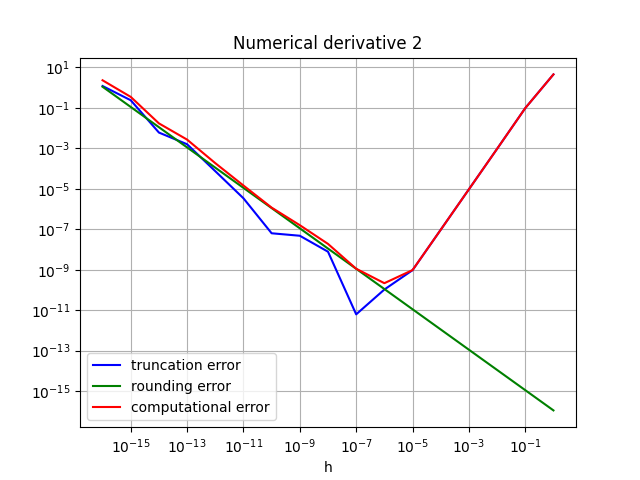
\includegraphics[width=\linewidth]{figures/numerical_derivative_2.png}
\end{figure}
\\
Wyznaczona wartość: $h_{min} = 10^{-6}$ \\
Wartość otrzymana ze wzoru $h_{min} \approx \sqrt[3]{3\cdot\epsilon/M}$,
gdzie $M \approx \left|f'''(x)\right|$: \\
$$M\approx \left|\frac{32\cdot cos^4(x)}{(1 + cos(2 x))^4} + \frac{16\cdot cos^2(x)\cdot sin^2(2 x)}{(1 + cos(2 x))^4}\right|
\approx 56.7$$

$$h_{min} \approx \sqrt[3]{3\cdot2^{-53}/56.7}
\approx 1.8 \cdot 10^{-6}$$
\\
Otrzymane wartości są tego samego rzędu wielkości.  \\
\\
\subsection*{Wnioski}
Z obliczeń wynika, że lepszą dokładność - mniejszą
wartość błędu obliczeniowego zapewniła druga 
wykorzystana metoda. \\
Wyznaczona wartość $h_{min}$ była bliższa wartości
obliczonej na podstawie wzoru dla drugiej metody.
\\

\section*{Zadanie 2.}
\textbf{Napisz program generujący pierwsze n wyrazów ciągu zdefiniowa-
nego równaniem różnicowym:
$$x_{k+1} = 2.25\cdot x_k - 0.5\cdot x_{k-1},$$
 gdzie $x_0 = \frac{1}{3}$, $ x_1 = \frac{1}{12}$.}
\\\\
Poniższy wykres przedstawia obliczone wartości 
kolejnych wyrazów ciągu dla reprezentacji liczb niecałkowitych 
korzystając z pojedynczej, podwójnej precyzji (odpowiednio
$numpy.single$ oraz $numpy.double$ z biblioteki $NumPy$) oraz z obiektów 
$Fraction$ z biblioteki $fractions$.
\begin{figure}[ht!]
    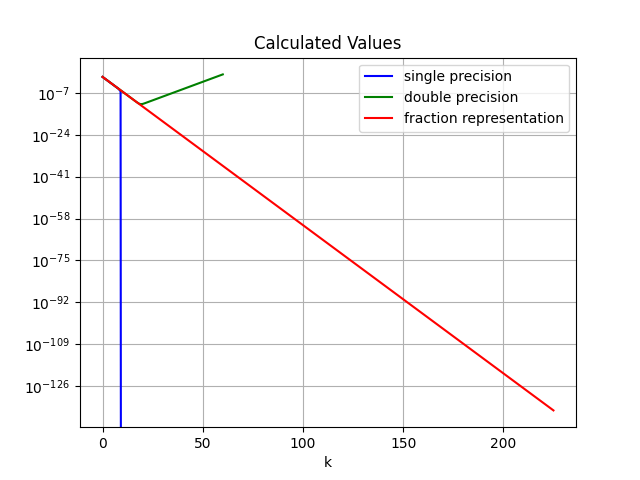
\includegraphics[width=\linewidth]{figures/calculated_values.png}
\end{figure}
\\
Poniższy wykres przedstawia obliczone wartości 
błędów względnych.
\begin{figure}[ht!]
    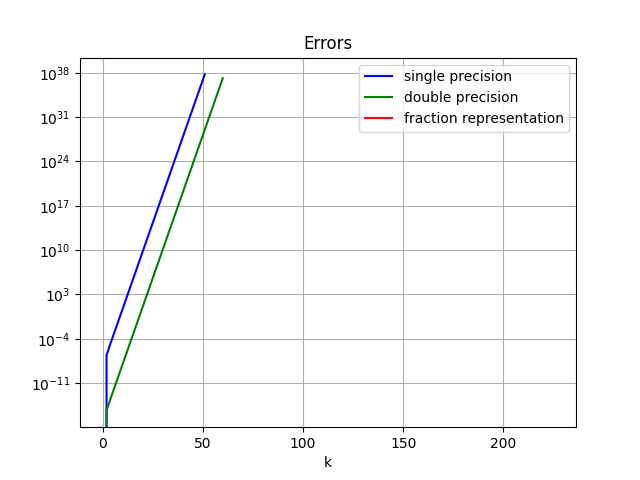
\includegraphics[width=\linewidth]{figures/errors.png}
\end{figure}
\\\\\\\\\\\\\\\\\\\\\\\\\\\\\\
\subsection*{Wnioski}
\quad Reprezentując liczby niecałkowite jako ułamki 
proste, kolejne wyrazy ciągu zachowywały się
tak samo jak wartości wyznaczone w sposób jawny.
Z tego powodu nie da się odczytać błędu korzystając ze
skali logarytmicznej - wynosi on 0. \\
\null\quad Pojedyncza precyzja - 32-bit'owa wersja float'a, przeznacza
23 bity na mantysę, co daje dokładność około 7.225 miejsc po przecinku. 
Jak można odczytać z wykresu - wartości pokrywają się z prawdziwymi mniej więcej do $x_k=10^{-7}$.
Próba obliczania kolejnych wartości powoduje, ze względu na niedokładności,
przejście na wartości ujemne, a następnie na wartość \textit{-inf} i wreszcie na
\textit{nan}, co prowadzi do wystąpienia \textit{overflow}\\
\null\quad Podwójna precyzja - 64-bit'owa wersja float'a, przeznacza
53 bity na mantysę, co daje dokładność około 15.955 miejsc po przecinku. 
Od elementów rzędu $10^{-11}$ wyrazy ciągu zaczynają rosnąć, zamiast maleć zgodnie z
tym jak powinien się zachowywać zadany ciąg. Wynika to z tego, że brak dokładności
w jednym z obliczeń kolejnego wyrazu ciągu powoduje, że element \textit{k+1}-szy,
ma wartość większą od elementu \textit{k}-tego, co powoduje zmianę kierunku
monotoniczności ciągu na przeciwny. \\



\section*{Źródła}
\begin{itemize}
    \item \url{https://en.wikipedia.org/wiki/Single-precision_floating-point_format}
    \item \url{https://en.wikipedia.org/wiki/Double-precision_floating-point_format}
\end{itemize}



\end{document}